%L'introduction est une section requise dans un rapport technique. Introduisez votre travail, l'idée de départ et les objectifs attendus. Un lecteur qui découvrirait votre projet au travers de cette introduction devrait ainsi être capable d'en comprendre le cadre, l'idée générale et les aboutissants du projet.
Dans le domaine de la santé, les nouveau-nés sont des patients requérant une attention particulière et un contrôle précis de leur 
paramètres vitaux. En effet, dès leur plus jeune âge, ils peuvent être victimes de plusieurs maladies dont les détresses respiratoires. 


\section{Contexte}
%Cette section \underline{n'est pas obligatoire}, mais elle est souvent présente dans un rapport technique pour compléter l'introduction et définir le contexte du travail \cad le cadre formel dans lequel le travail est mené.
Dans le domaine médical, plusieurs appareils de monitoring sont utilisés afin de contrôler les paramètres vitaux des patients. 
Selon le type de patient, les appareils utilisés sont différents. En effet, un nouveau-né a un comportement différent d'une personne 
adulte. Il est alors nécessaire de contrôler ces paramètres vitaux à l'aide d'appareils adaptés. \\
Ce Travail de Bachelor porte sur un débitmètre respiratoire innovant. Ce dernier permettrait de calculer le flux d'air entrant et sortant
du patient et, ainsi, de contrôler son débit respiratoire. 
\section{Etat de l'art}
\subsection{Débitmètre néonataux sur le marché}
\begin{comment}
Actuellement, ce qui existe sur le marché sont des anémomètres à double fils chauds (double hot wire anemometer). Ces débitmètre 
mesure le flux des patients néonataux. \\
Les revues scientifiques parlent également de débitmètre pédiatrique. Leur fonctionnement  
\end{comment}
Plusieurs entreprises proposent des débitmètre néonataux. Ces entreprises ont été regroupées dans le tableau ci-dessous avec les 
techniques utilisées. \\

\begin{centering}
    \begin{tabular}{|c|c|}
        \hline
        Entreprises & Technologie                         \\
        \hline
        Sensirion   & Capteur thermique de débit massique \\
        \hline
        Mim-Germany & Anémomètre à fil chaud double       \\
        \hline
        Europlaz    &                                     \\
        \hline
        Draeger     & Anémomètre à fil chaud              \\
        \hline
        \label{tab:marques}
    \end{tabular}
\end{centering}


\subsection{Revues scientifiques}
Les revues scientifiques sont également des ressources intéressantes à considérer pour l'élaboration de l'état de l'art. En effet, les 
articles scientifiques vont permettre d'établir une liste des techniques déjà exploitées, leur fonctionnement plus en détail ainsi que leurs 
performances. \\
\begin{figure}[H]
    \centering
    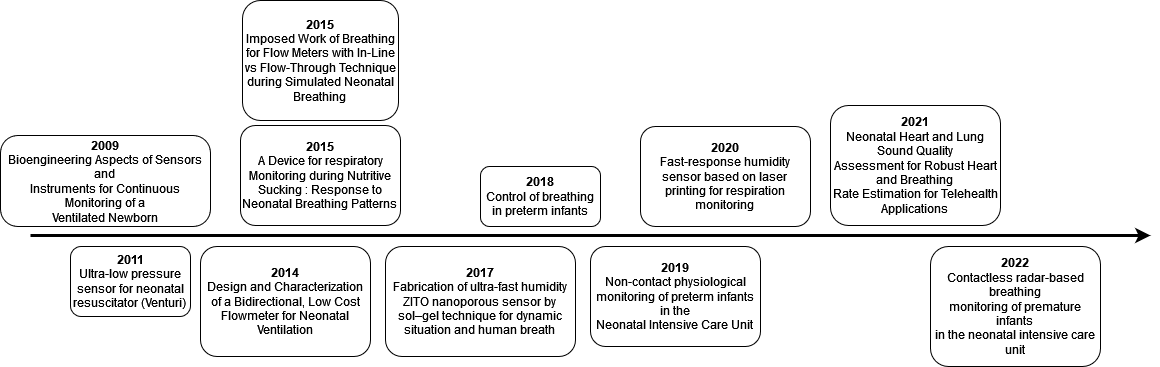
\includegraphics[scale = 0.3]{images/DRP_Etat_de_l_art.png}
    \caption{Articles scientifiques par ordre chronologique}
    \label{fig:articlesChrono}
\end{figure}

Les articles pertinants pour ce Travail de Bachelor sont résumés dans ce chapitre et classé par ordre chronologique sur la figure 
\ref{fig:articlesChrono}. \\

Le premier article \cite{rolfe_bioengineering_2009}, mentionne plusieurs débitmètres différents. Le pneumotacographe de Fleisch, par exemple, est un 
système par lequel le débit repiratoire est mesuré grâce à une différence de pression. Cette différence de pression est engendré par 
un rétrécissement de l'espace de circulation du gaz (principe de Venturi) \cite{oberg_biomedical_2011}. \\

Par la suite, il est expliqué que le pneumotachographe est gentiment remplacé par les anémomètres à fil chaud. Ces capteurs sont 
constitués d'un ou plusieurs fils chauffé par une source de courant. Lorsqu'un flux d'air va souffler sur le fil, la chaleur sera 
transférée du fil au gaz. Le capteur viendra alors mesurer la quantité de chaleur transférée ainsi que la différence de température entre 
le fil et le gaz pour finalement calculer le débit \cite{oberg_biomedical_2011}. \\
L'article sus-mentionné conseil l'utilisation des anémomètres à plusieurs fils contrairement à ceux à un seul fil qui aurait des performances 
moindres. 
L'anémomètre à fils chauds est une technologie incorporée par exemple dans la machine "Draeger Babylog", marque mentionnée dans le tableau \ref{tab:marques}. \\

Le second article exploite le principe de Venturi mentionné auparavant \cite{jacq_ultra-low_2011}. Il est destiné à une aplication 
quelques peu différente puisqu'il est  intégrer dans un ressuscitateur. Un tel appareil permet la réanimation du patient qui ne respire 
plus. Le ressuscitateur gonfle les poumons d'air et ainsi s'assure qu'un bon taux d'oxygène circule dans le patient. \\
Pour les nouveaux-né, la quantité d'air injectée dans les poumons doit être mesurée car un trop grand débit pourrait rapidement engendrer 
des dégats. \\
Couplé au système de Venturi, un capteur de force vient mesurer la pression et le volume d'air passant par le ressuscitateur. \\

Une autre technologie pour débitmètre consiste à utiliser le transfert de chaleur entre deux transistors. 
\begin{figure}[H]
    \centering
    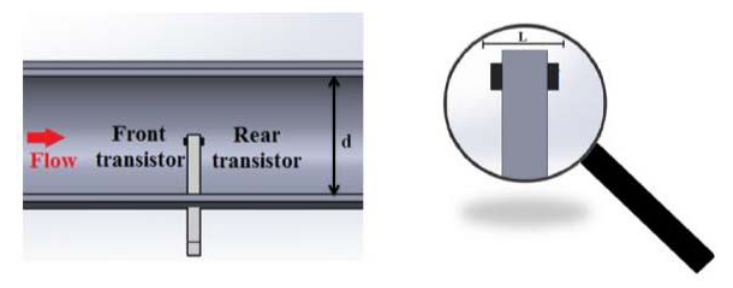
\includegraphics[scale = 0.5]{images/Debitmetre_transistors.png}
    \caption{Principe du débitmètre à transistors}
    \label{fig:transistors}
\end{figure}
C'est un principe encore innovant décrit dans l'article \cite{giorgino_design_2014} et utilisé dans l'article \cite{rosi_device_2016}. 
Le premier transistor est placé perpendiculairement au flux d'air sur un PCB. \\
Le second est fixé de l'autre côté du PCB dos à dos avec le premier transistor (cf. figure \ref{fig:transistors}). \\
De cette manière, le capteur sera capable de distinguer une expiration d'une inspiration. Le temps de réponse d'un tel capteur serait 
d'environ 340ms. C'est un très bon temps de réponse en comparaison des capteurs médicaux existants sur le marché. Cependant, diverses améliorations 
doivent encore être faites avant de pouvoir utiliser une telle technologie. \\

\begin{comment}
L'article suivant est intéressant au niveau du listage des débitmètres pédiatriques existants \cite{}. En effet, il étudie les différents fonctionnements 
existants et compare les signaux obtenus. Étant donné que cet article étudie plus précisément une caractéristique ("IN-line" vs "Flow-Through"), 
il est moins important dans le cadre de ce projet.\\
\end{comment}

Un autre article mentionne les membranes nanoporeuses comme capteur \cite{moharamzadeh_fabrication_2018}. Cependant, ces capteurs sont pour l'humidité et non le débit 
respiratoire. Des nanostructures d'oxyde de Zinc sont utilisées, car elles possèdes de bonnes propriétés physiques et chimiques. Bien que l'humidit 
et le débit respiratoire soient en lien, l'article n'a pas étudiés en détail l'application de cette membrane au débit respiratoire directement. \\
Cependant, un temps de réponse plutôt bon, de l'ordre de la seconde est attendu avec une telle technologie. \\

Le prochain article repose sur une technologie de monitoring non-invasive. Elle utilise une caméra qui suit les mouvements du nouveaux-né. 
Cette technologie permet également d'enregistrer d'autres signaux tels que la fréquence cardiaque mais elle requiert encore quelques améliorations 
ainsi que quelques recherches supplémentaires. 


\section{Un débitmètre innovant}
Ce travail de Bachelor est une recherche à propos d'un débitmètre dont le principe de fonctionnement est encore innovant. Il utilise des 
membranes nanoporeuses qui permettent une acquisition de données rapides. 

\section{Fonctionnement du débitmètre respiratoire pédiatrique}
Le capteur développé lors de ce Travail de Bachelor, comme évoqué plus haut, repose sur une membrane nanoporeuse achetée sur le marché. 
Un côté de la membrane va être recouverte d'un matériau conducteur, l'or. Puis, Les pores de cette membrane sont remplies par 
électrodéposition avec une solution de Tellure de Bismuth (cf. figure \ref{fig:electrodeposition}). 
\begin{figure}[H]
    \centering
    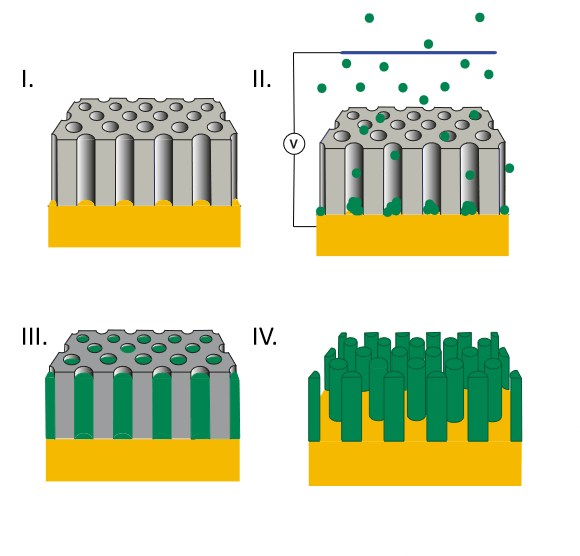
\includegraphics[scale = 0.5]{images/Electrodeposition.png}
    \caption{Electrodéposition \cite{ruiz-gomez_electrodeposition_2022}}
    \label{fig:electrodeposition}
\end{figure}

Par la suite, ces étape seront répétées une seconde fois afin d'obtenir le capteur suivant :  
\begin{figure}[H]
    \centering
    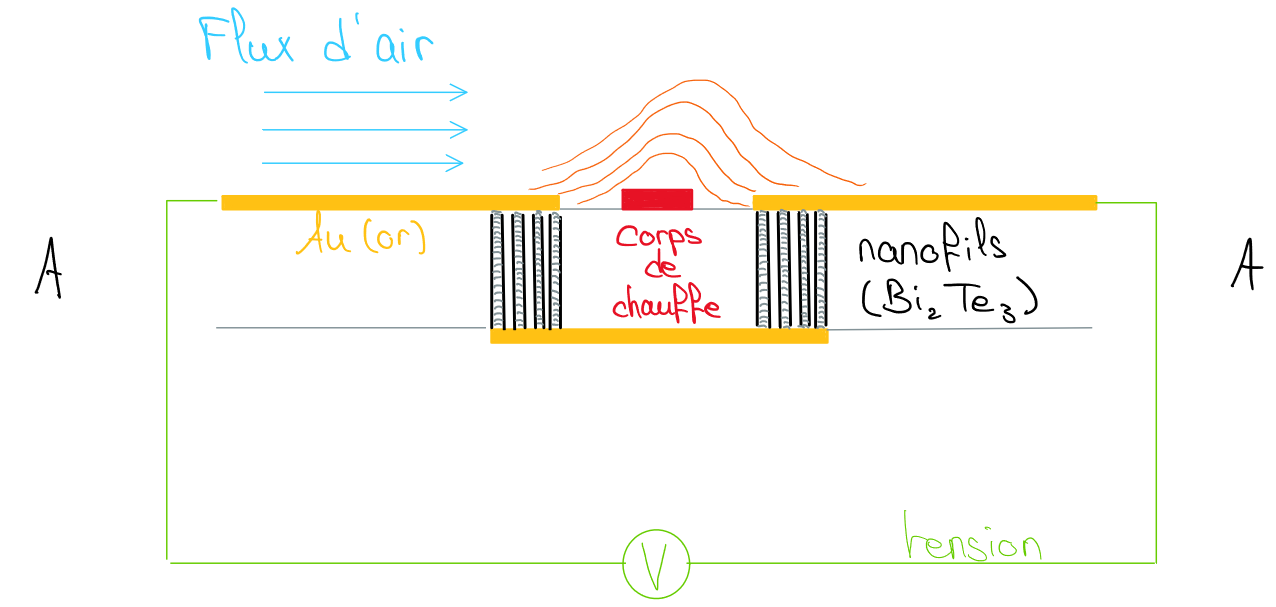
\includegraphics[scale = 0.5]{images/CapteurFUN.png}
    \caption{Capteur par membranes nanoporeuses}
    \label{fig:capteurFUN}
\end{figure}

La couche d'or en dessous du capteur permet de court-circuiter les deux membranes ensembles. \\
Un corps de chauffe est placé entre les deux membranes nanoporeuses. Une différence de température entre ces membranes va se créer 
lorsque le patient viendra expirer ou inspirer de l'air sur le corps de chauffe. \\
Avec cette différence de température de part et d'autre du dispositif, une tension va apparaître. Il sera alors possible de lier 
cette tension au débit inspiré et expiré du nouveau-né.\\

\section{Cahier des charges}

\section{Livrables}

\section{Planification}

\section{Plan du rapport}

%%if
\section{Citations et bibliographie}
Citer vos sources est essentiel. Avec \texttt{biblatex} vous pouvez facilement citer des articles, des livres ou des sites internet. Toutes les citations dans le texte seront automatiquement regroupées en fin de document dans la section \guillemotleft Bibliographie\guillemotright. Par exemple, citons un article d'Einstein \cite{einstein} ou le livre de Dirac \cite{dirac}.

Parfois il peut être utile d'utiliser un gestionnaire de bibliographie. La communauté académique recommande l'outil \href{https://www.zotero.org/}{Zotero} qui permet de gérer une bibliothèque numérique d'ouvrages et de références numériques. Il permet également de générer une bibliographie compatible avec \LaTeX.

Notez qu'il est très facile d'obtenir l'extrait \texttt{bibtex} depuis des journaux. Sélectionnez \emph{export/citation}. Si vous le pouvez choisissez \texttt{bibtex}. Dans le cas d'un format \texttt{.ris}, utilisez un convertisseur en ligne comme \href{http://www.bruot.org/ris2bib/}{ris2bib}.

\section{Adapter votre modèle}
Ce document n'est qu'un modèle ayant pour but de revoir les quelques avantages de \LaTeX~ et les fonctionnalités qui pourraient vous être utiles pour rédiger un rapport académique. N'hésitez pas à supprimer les parties inutiles et à adapter ce modèle à vos besoins.
%%fi